\chapter{Analysis} \label{Analysis}

%TODO: edit this awkwardness
This tool will be analyzed by looking at three case studies. 
We created three instrument types: Spectrometer, High Resolution Spectrometer, and FX Correlator, as defined in Sections \ref{Real Time Radio Astronomy Algorithms:Spectroscopy}, \ref{Real Time Radio Astronomy Algorithms:Pulsar Processing}, and \ref{Real Time Radio Astronomy Algorithms:Correlation}. 
Each instrument type has a set of parameters relevant to that instrument. 
Additional instruments or new parameters for existing instruments can be added by defining how those parameters affect the final dataflow diagram. 
This translation is described further in the next section.


%Summary: describe how we get real numbers to put into previous part
%Goal: define and obtain real numbers from the previous part
%\section{Benchmarks}


%\subsection{Cost}





%Summary: case studies describing partitioning of realistic-scale instruments
%Goal: show successful application of tool to design of realistic instruments
%provide analysis comparing this to hand-designed instruments 
\section{Spectrometer Case Study}

\subsubsection{Spectrometer Definition}
Defining a simple spectrometer requires very few parameters. 
First, as with most instruments, the astronomer must specify the sky bandwidth the instrument must process, defined in MHz.
Then, the desired spectral resolution is defined in MHz per channel, or analogously, the number of channels that should be used to break up the bandwidth.
Finally, the integration time needs to be defined.

One optional parameter, number of antennas, can also be defined. 
This describes the number of independent spectrometers that need to be created.
While this parameter does not affect the end to end processing for each antenna, knowing how many spectrometers are needed allows for more efficient use of the hardware.
The impact on the design is described further in Sections \ref{High Level Toolflow:Dataflow Model} and \ref{High Level Toolflow:Mapping} and the cost efficiency afforded by this parameter is explored in Chapter \ref{Analysis}

Simple spectrometer placement

Include appropriate FFT or PFB benchmarks

\subsubsection{Spectrometer}

\begin{figure}[ht!]
  \centering
    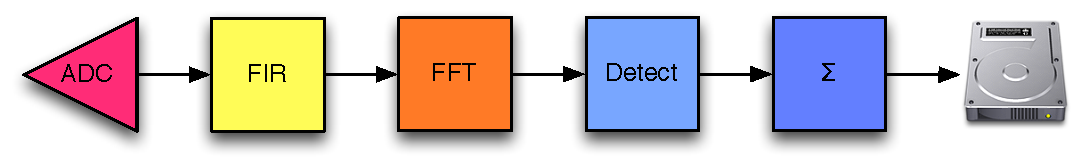
\includegraphics[width=1\textwidth]{Images/C4/spectrometer_dataflow.pdf}
  \caption[General Spectrometer Dataflow Model]{General Spectrometer Dataflow Model.
  \textit{
  A general dataflow model for a single antenna spectrometer. 
  This model can be applied to any spectrometer, as the spectrometer parameters do not affect how many computational blocks are required or the interconnect layout. 
  %TODO: This is questionable, ask dan
  The data is fed in by an ADC and filtered using an FIR to improve the response of the FFT.
  The filtered data is then channelized by an FFT, accumulated in the block labeled $\Sigma$ and recorded to disk.
  }}
  \label{fig: C4/spectrometer_dataflow.pdf}
\end{figure}

The spectrometer instrument definition generates a very simple dataflow. 
Figure \ref{fig: C4/spectrometer_dataflow.pdf} shows the general dataflow model for a spectrometer. 
The ADC feeds data into a FIR filter. 
Then the filtered signal is transformed into channels in the FFT and those channels are accumulated and saved to disk. Regardless of the parameters the astronomer chooses, the dataflow will be the same. 

The parameters for each block come directly from the instrument definition. 
The FIR parameters come from the number of FIR taps and window shape, the FFT is simply defined by the FFT length parameter and the accumulator also is parameterized by the FFT length as well as the integration time. 

\subsection{Cost}
\subsection{Power}

\section{High Resolution Spectrometer Case Study}
\subsubsection{High Resolution Spectrometer Definition}
The main difference between a spectrometer and a high resolution spectrometer is the need for two stages of channelization rather than just one. 
The sky bandwidth, integration time, and number of antennas are defined in the same way as the previous spectrometer type. 

The spectral resolution is defined differently, because both the coarse and fine resolutions need to be defined. 
The coarse resolution defines how many channels the whole sky bandwidth should be broken up into initially.
The fine resolution defines how many channels each coarse channel is broken into.
Both can be described in MHz per channel.

\subsubsection{High Resolution Spectrometer Dataflow}

\begin{figure}[ht!]
  \centering
    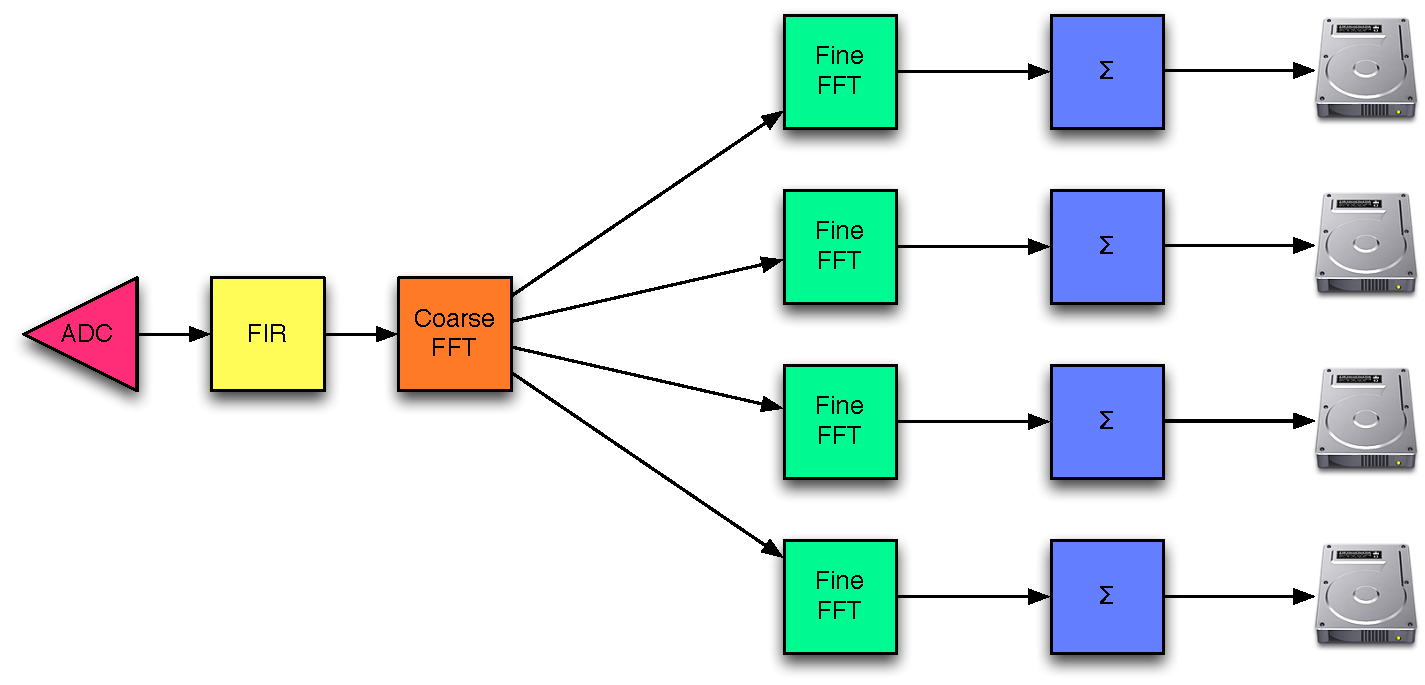
\includegraphics[width=1\textwidth]{Images/C4/hires_spectrometer_dataflow.pdf}
  \caption[Example High Resolution Spectrometer Dataflow Model]{Example High Resolution Spectrometer Dataflow Model
  \textit{
  This figure shows an example dataflow for a high resolution spectrometer with 4 coarse FFT channels.
  Like the previous spectrometer, the data comes in through an ADC, is filtered and then channelized using a coarse FFT.
  Then, to achieve a higher resolution, each coarse channel is divided into sub-channels using the 4 fine FFT blocks in the dataflow. 
  }}

  \label{fig: C4/hires_spectrometer_dataflow.pdf}
\end{figure}

The high resolution spectrometer dataflow does depend on the parameters specified in the instrument description. 
An example dataflow is shown in Figure \ref{fig: C4/hires_spectrometer_dataflow.pdf}. 
The first three blocks in the dataflow are exactly the same as the Spectrometer dataflow described in the previous section. 
An ADC feeds data into a FIR filter followed by an FFT. 
After the FFT, the algorithm is modified to accommodate the higher resolution required. 
The first FFT divides the band into a number of coarse channels and then each coarse channel must be further divided into a number of fine channels. 
The coarse FFT must feed its data to a separate fine FFT for each coarse channel, so the number of fine FFTs in the dataflow diagram will vary based on the number of coarse channels.
At this point, each coarse channel is processed in an independent pipeline the finely channelized data is accumulated and recorded to disk. 
The example in Figure \ref{fig: C4/hires_spectrometer_dataflow.pdf} shows a spectrometer that divides the data into 4 coarse channels.

results for hi res spectrometer (gbt and seti)

Serendip 6 300MHz 7 ant 2 pol

1Hz resolution (256 million channels)

Greenbank 2.5GHz 1 beam 2 pols

1 Hz resolution

Same benchmarks as before, just discuss large bw, multi stage fft
\subsection{Cost}
\subsection{Power}
\subsection{Algorithmic Exploration}

\section{FX Correlator Case Study}
\subsubsection{FX Correlator Definition}
An FX Correlator is also defined by the amount of bandwidth it processes, number of channels, and integration time, but now the number of antennas is a necessary parameter.

\subsubsection{FX Correlator Dataflow}

The FX dataflow model is based on the algorithm used by the CASPER correlator described in Section \ref{Related Work:Radio Astronomy}. The processing model is described by replicating 2 basic pipelines, called an F-Engine and an X-Engine. The number of times each pipeline needs to be replicated depends on the number of antennas and number of channels this correlator requires.

\begin{figure}[h!]
  \centering
    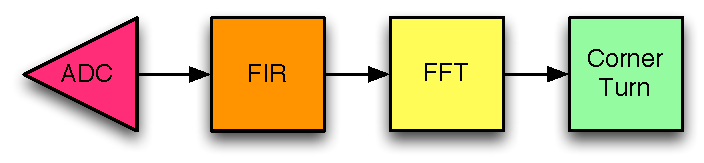
\includegraphics[width=0.48\textwidth]{Images/C4/fx_f_engine.pdf}
  \caption{FX Correlator F-Engine Model}
  \label{fig: C4/fx_f_engine.pdf}
\end{figure}

An F-Engine, pictured in Figure \ref{fig: C4/fx_f_engine.pdf} is responsible for channelizing the data from a single antenna. 
It takes in data from an ADC, and channelizes the data using a FIR and FFT to create a polyphase filter bank. 
The number of F-Engines in the correlator dataflow will vary with the number of antennas.

\begin{figure}[h!]
  \centering
    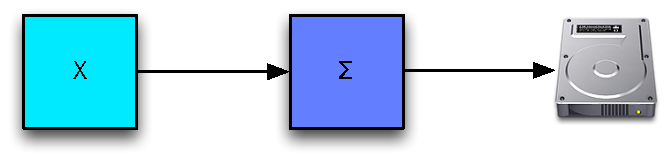
\includegraphics[width=0.48\textwidth]{Images/C4/fx_x_engine.pdf}
  \caption{FX Correlator X-Engine Model}
  \label{fig: C4/fx_x_engine.pdf}
\end{figure}

The second pipeline, the X-Engine processes the channelized data. 
Each X-Engine takes a single channel of data from every antenna in the array, cross-correlates the data, accumulates it and stores it to disk. 
Figure \ref{fig: C4/fx_x_engine.pdf} shows the pipeline for a single X-Engine. 
Since each X-Engine only operates on a single channel, the total number of X-Engines in the correlator must be the same as the number of channels in the FFT.

\begin{figure}[h!]
  \centering
    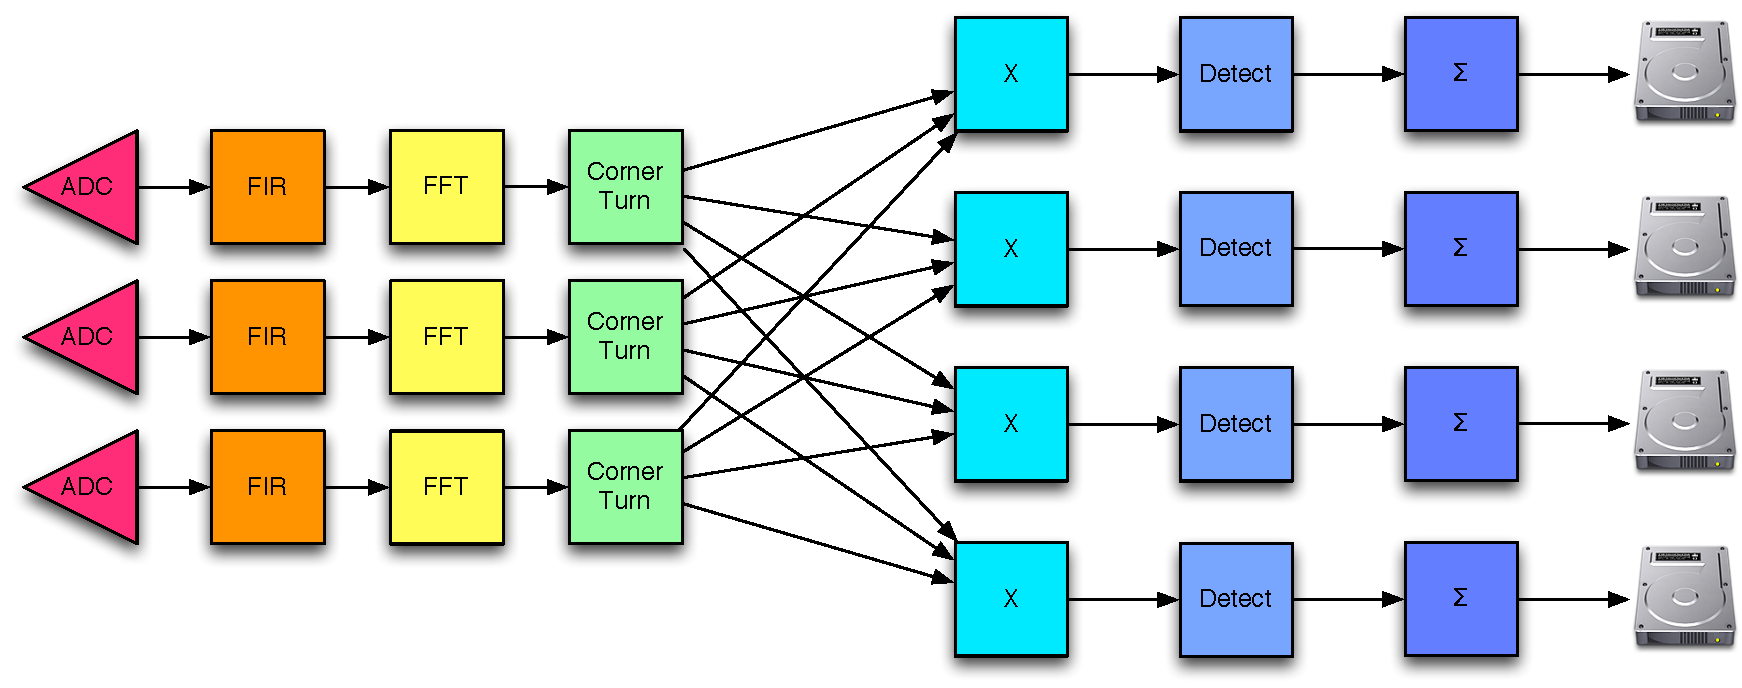
\includegraphics[width=1\textwidth]{Images/C4/fx_dataflow.pdf}
  \caption{Example FX Correlator Dataflow Model}
  \label{fig: C4/fx_dataflow.pdf}
\end{figure}

The dataflow for an FX correlator will vary quite a bit based on the input parameters. 
Figure \ref{fig: C4/fx_dataflow.pdf} shows an example there antenna four channel FX correlator. 
The left half of the figure has three F-engines, for each of the three antennas.
The right half has four X-engines, one for each channel.
And in the center, since each X-engine requires data from every F-engine, the cross-correlation blocks, represented by an \emph{X} and the FFT blocks are connected in an all-to-all configuration.



xgpu benchmarks, correlator placement

Need benchmarks for xengine

HERA Correlator

572 ant dual pol (currently can run in under 5 minutes)

100 MHz

1024 channels

FPGA F, xGPU X

LWA @ OVRO

10k ant dual pol

120k signals

60MHz

4096 channels

1MWatt est w/GPU x-engine

SKA

4000 ant (8k signals)

10 GHz

16k channels




\subsection{Cost}
\subsection{Power}

\section{Model Scaling}
What about really big stuff?

\section{Mixed Cost Models}
Discuss mixing power+price
